\documentclass{standalone}
\usepackage{tikz}
\usepackage{ctex,siunitx}
\setCJKmainfont{Noto Serif CJK SC}
\usepackage{tkz-euclide}
\usepackage{amsmath}
\usepackage{wasysym}
\usetikzlibrary{patterns, calc}
\usetikzlibrary {decorations.pathmorphing, decorations.pathreplacing, decorations.shapes}
\newcommand{\posthead}[2][gray]{
  \begin{scope}[#2]
    \fill[left color=#1,right color= #1,middle color=#1!20](0,0)ellipse(0.05 and 0.02);
    \fill[left color=#1,right color= #1,middle color=#1!20](0.05,0)rectangle(-0.05,0.07);
    \fill[left color=#1,right color= #1,middle color=#1!20](-0.06,0.07)arc(-180:0:0.06 and 0.02)--(0.06,0.15)--(0.05,0.16)--(-0.05,0.16)--(-0.06,0.15)--cycle;
    \fill[#1!50!gray](0,0.16)ellipse(0.05 and 0.02);
    \foreach \x in {75,45,15,-15,-45,-75}
    {
      \draw[very thin,#1!50!gray]({0.05*sin(\x)},{0.16-0.02*cos(\x)})--({0.06*sin(\x)},{0.15-0.02*cos(\x)})--++(0,-0.08);
    }
  \end{scope}
}
\begin{document}
\small
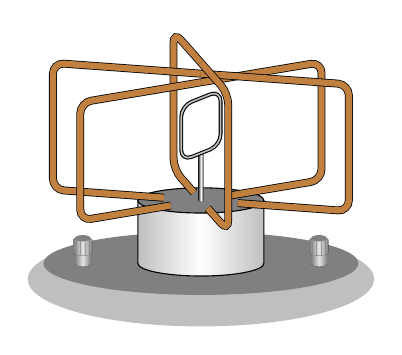
\begin{tikzpicture}[>=latex,scale=1.0]
  % \useasboundingbox(0.9,0)rectangle(5.1,5);
  \fill[lightgray](0,-0.2)ellipse(2.2 and 0.6);
  \fill[gray](0,0)ellipse(2 and 0.4);
  \posthead{xshift=1.5cm,scale=2}
  \posthead{xshift=-1.5cm,scale=2}
  \draw[left color=lightgray,right color=lightgray,middle color=white](-0.8,0.8)--(-0.8,0)arc(-180:0:0.8 and 0.16)--(0.8,0.8)--cycle;
  \draw[fill=gray](0,0.8)ellipse(0.8 and 0.16);
  \fill[left color=darkgray,right color=darkgray,middle color=white](-0.03,1.4)--(-0.03,0.8)arc(-180:0:0.03 and 0.016)--(0.03,1.4)--cycle;
  \foreach \x/\y in {100/0.25,40/0,160/0.11}
  {\draw[double=brown,double distance=0.8mm,rounded corners,line width =0.1mm]({0.5*cos(\x)},{0.8+0.1*sin(\x)})--++({1.5*cos(\x)},{0.3*sin(\x)})--++(0,1.5+\y)--++({2*cos(180+\x)},{0.4*sin(180+\x)});}
  \draw[double=lightgray,rounded corners](0,1.4)--++(0.25,0.1)--++(0,0.7)--++(-0.5,-0.2)--++(0,-0.7)--cycle;
  \foreach \x/\y in {220/0,340/0.11,280/0.25}
  {\draw[double=brown,double distance=0.8mm,rounded corners,line width =0.1mm]({0.5*cos(\x)},{0.8+0.1*sin(\x)})--++({1.5*cos(\x)},{0.3*sin(\x)})--++(0,1.5+\y)--++({2*cos(180+\x)},{0.4*sin(180+\x)});}
\end{tikzpicture}
\end{document}